
\documentclass[a4paper,11pt]{article}


%%% fontenc
%\usepackage{fontspec,xunicode,xltxtra}
%\setmainfont{Times New Roman}
%\setsansfont{Source Sans Pro}
%\setmonofont{Source Sans Pro}

%%% xeCJK
\usepackage{xeCJK}
\setCJKmainfont[BoldFont=Adobe Heiti Std]{Adobe Song Std}
\setCJKsansfont[BoldFont=Adobe Heiti Std]{Adobe Song Std}
\setCJKmonofont[BoldFont=Adobe Heiti Std]{Adobe Song Std}
\XeTeXlinebreaklocale "zh"
\XeTeXlinebreakskip=0pt plus 1pt minus 0.1pt

\usepackage{xcolor}
\usepackage{graphicx}

%%% get total page number
\usepackage{lastpage}

%%% customized definition
\makeatletter
\def\sybtitle#1{\def\@sybtitle{#1}}
\def\sybauthor#1{\def\@sybauthor{#1}}
\def\sybdate#1{\def\@sybdate{#1}}
\sybtitle{}
\sybauthor{}
\sybdate{}
\def\sybmaketitle{
  \begin{center}
  \vspace*{.8in}
  {\huge\bfseries\@sybtitle}
  \par
  \vspace{.8in}
  {\Large\@sybauthor}
  \par
  \vspace{.2in}
  \@sybdate
  \vspace{.5in}
  \end{center}
}
\makeatother
\setlength{\parindent}{0pt}
\renewcommand{\today}{\number\month 月 \number\day 日, ~\number\year 年}
\def\lt{\textless}
\def\gt{\textgreater}
\renewcommand\contentsname{\bfseries 目~~录}
\newcommand\bs{\texttt{\symbol{'134}}} % input backslash sign
%\newcommand\bs{\string\} % same as above definition
\long\def\cmd#1{\par\vspace{.5em}\hspace*{2em}#1\vspace{.5em}\par}
\def\cstr#1{\texttt{\string#1}} % e.g. \cstr{\latex}
\long\def\runcode#1{\par\bigskip#1\bigskip\par}
% 我不想看到那么多的underful hbox,尤其是minted环境加上背景色之后
\hbadness=10000
% 适当放宽overful hbox的限制,运行2pt的溢出
\hfuzz=2pt
\parskip=3\lineskip


%%% change background color & add frame for enumerate enviroment
\usepackage{mdframed}
\newmdenv[backgroundcolor=blue!10,linewidth=0pt]{coloredframe}
\newenvironment{coloredenumerate}{
  \begin{coloredframe}
  \begin{enumerate}
}{
  \end{enumerate}
  \end{coloredframe}
}

%%% geometry
\usepackage[includehead,includefoot,hmargin=21mm,vmargin=10.5mm,
            headsep=12pt,headheight=25pt]{geometry}
%\usepackage[includehead,includefoot,hmargin=1.2in,vmargin=1in]{geometry}

%%% fancyhdr
\usepackage{fancyhdr}
\makeatletter
\fancypagestyle{main} {
  \fancyhf{} % clear header & footer
  \fancyhead[L]{\bfseries\@sybtitle}
  \fancyhead[R]{\thepage/\pageref*{LastPage}}
  \renewcommand{\headrulewidth}{0.4pt} % header line
  \renewcommand{\footrulewidth}{0pt} % footer line
}
\fancypagestyle{header} {
  \fancyhf{} % clear header & footer
  \fancyfoot[C]{\roman{page}}
  \renewcommand{\headrulewidth}{0pt} % header line
  \renewcommand{\footrulewidth}{0pt} % footer line
}
\makeatother

\usepackage{titlesec}
\titleformat{\part}{\centering\Large\bfseries}{第\,\thepart\,部分}{1em}{}
\titleformat{\section}{\large\bfseries}{\thesection}{1em}{}
\titleformat{\subsection}{\normalsize\bfseries}{\thesubsection}{1em}{}
%\titlespacing*{章节命令}{左边距}{上文距}{下文距}[右边距]
\titlespacing*{\section}{0pt}{2\baselineskip}{\parsep}


\usepackage{hyperref}

%%% perfect source code display
\usepackage{minted}
%\usemintedstyle{colorful}
\definecolor{srcbg}{rgb}{0.95,0.95,0.95}
\newminted{java}{linenos,tabsize=4,bgcolor=srcbg}
\newminted{xml}{linenos,tabsize=4,bgcolor=srcbg}
\newminted{cpp}{linenos,tabsize=4,bgcolor=srcbg}
\newminted{bash}{linenos,tabsize=4,bgcolor=srcbg}
\newminted{latex}{linenos,tabsize=4,bgcolor=srcbg}
\newminted{scheme}{linenos,tabsize=4,bgcolor=srcbg}

\usepackage{amsmath}


\input{../styles/tikz_preamble}

\sybtitle{Concurrency and Parallel}
\sybauthor{孙延宾}
\sybdate{\today}

\begin{document}
\tt % I love Typewriter font.
%%%%%%%% the title page and toc %%%%%%%%%%
\pagestyle{header}
\sybmaketitle
%\tableofcontents
\newpage

%%%%%%% the main content %%%%%%%%%
\pagestyle{main}
\setcounter{page}{1}

\section[什么是并发?]{什么是并发?}
Concurrency,并发性,是指两个或者多个事件在一个时间间隔内同时发生。

并发性的重点是“一个时间间隔”,即我们说两个或者多个事件是否是并发的,
需要考察“一段时间”而非某一个“时刻”。如我们考察A、B两个事件的并发性,
\begin{itemize}
  \item 首先选定一个时间段,时长可能是1小时,可能是1分钟,也可能是1纳秒;
  \item 然后再看在这段时间内,A、B是否都发生了,至于发生顺序则不用关注。
\end{itemize}
并发性并不关注事件是如何发生的,A、B并发,可能A先发生B后发生,
也可能反着,也可能A、B交替发生,还有可能A、B始终同时发生(任一时刻A、B
都在发生)或者一段时间内同时发生一段时间内交替发生,这些我们都不关注,
他们不影响并发性的判定。

\section[什么是并行?]{什么是并行}
Parallel,并行性,是指两个或者多个事件在同一时刻发生。

并行性的重点是“同一时刻”,即一段时间内的任一时刻,两个或者多个事件
都在发生,则说这段时间内这些事件是并行的,当然这里仍然需要确定一个
时间段才行。

“同一时刻”多个事件都发生,说明这些事件具有同时性。

\section[并发与并行的区别]{并发与并行的区别}
从上面的介绍可以看出,无论是并发还是并行都需要明确一个时间段,
然后才能说这个时间段内,多个事件是并发的还是并行的。

并发跟并行比较,可以看出并发比并行的范围更广,即并行一定是并发,
但是反之则不一定成立。

\begin{center}
  \emph{并行性=并发性+同时性}
\end{center}

一段时间内多个事件并发,
有可能这段时间内的任一时刻,这些事件都在发生,于是这段时间内这些
事件就不只是并发了,他们还是并行的。

\begin{figure}
  \centering
  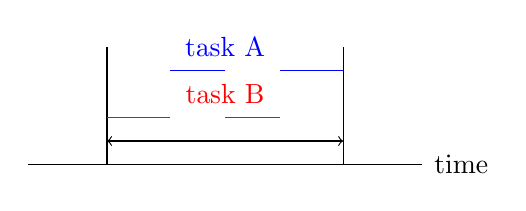
\begin{tikzpicture}
  \coordinate (origin) at (0,0);
  \coordinate (start) at (1cm, 0);
  \coordinate (end) at (4cm, 0);
  \coordinate (infinity) at (5cm, 0);
  
  \path (origin) edge (infinity);
  \node () at ([xshift=.5cm]infinity) {time};
  \draw (start) -- ([yshift=1.5cm]start);
  \draw (end) -- ([yshift=1.5cm]end);
  \draw[<->] ([yshift=.3cm]start) -- ([yshift=.3cm]end);
  
  \draw[color=red] ([yshift=.6cm]start) -- ([xshift=.8cm, yshift=.6cm]start);
  \draw[color=red] ([xshift=1.5cm, yshift=.6cm]start) -- ([xshift=2.2cm, yshift=.6cm]start);
  
  \draw[color=blue] ([xshift=.8cm, yshift=1.2cm]start) -- ([xshift=1.5cm, yshift=1.2cm]start);
  \draw[color=blue] ([xshift=2.2cm, yshift=1.2cm]start) -- ([xshift=3cm, yshift=1.2cm]start);
  
  \node[color=red] at (2.5cm, .9cm) {task B};
  \node[color=blue] at (2.5cm, 1.5cm) {task A};
  
  \end{tikzpicture}
  \caption{并发,但不限于此}\label{fig:concurrency}
\end{figure}

\begin{figure}
  \centering
  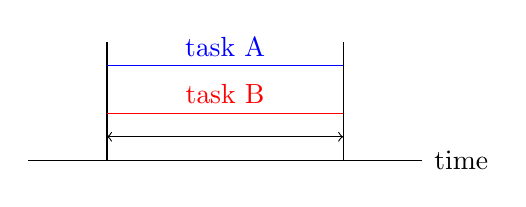
\begin{tikzpicture}
  \coordinate (origin) at (0,0);
  \coordinate (start) at (1cm, 0);
  \coordinate (end) at (4cm, 0);
  \coordinate (infinity) at (5cm, 0);

  \path (origin) edge (infinity);
  \node () at ([xshift=.5cm]infinity) {time};
  \draw (start) -- ([yshift=1.5cm]start);
  \draw (end) -- ([yshift=1.5cm]end);
  \draw[<->] ([yshift=.3cm]start) -- ([yshift=.3cm]end);
  
  \draw[color=red] ([yshift=.6cm]start) -- node[above] {task B} ([yshift=.6cm]end);
  \draw[color=blue] ([yshift=1.2cm]start) -- node[above] {task A} ([yshift=1.2cm]end);
  \end{tikzpicture}
  \caption{并行,且仅此一种}\label{fig:concurrency}
\end{figure}

\end{document}